\chapter{Gruppen verwalten}\label{gruppenVerwalten}
\minitoc
\clearpage


\section{Gruppen verwalten}
\begin{figure}[ht]
	\centering
	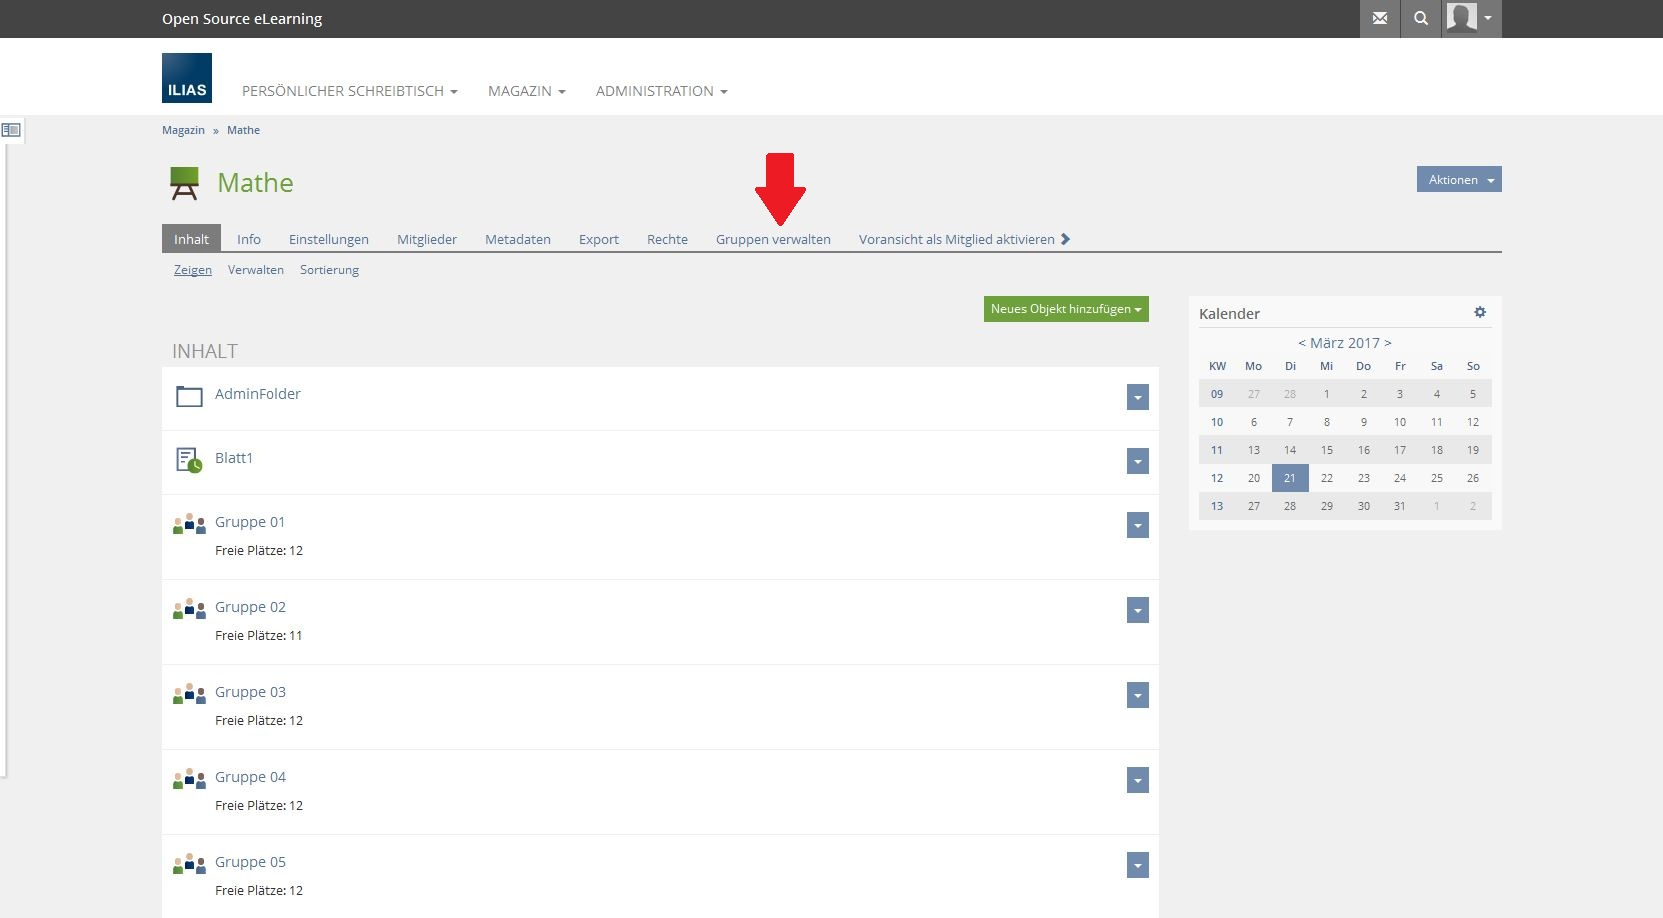
\includegraphics[width=1\textwidth]{img/gruppenverwalten.jpg}
	\caption{Ansicht Tab Gruppen verwalten im jeweiligen Kurs}
\end{figure}
\clearpage


\section{Gruppen erstellen}
\begin{figure}[h!]
	\centering
	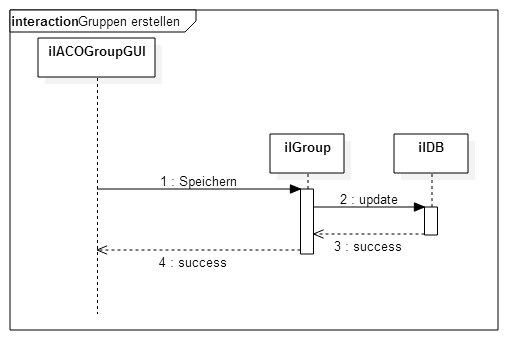
\includegraphics[width=.75\textwidth]{img/seq_groupGUI.png}
	\caption{Sequenzdiagramm Gruppen erstellen}
\end{figure}
\begin{figure}[h!]
	\centering
	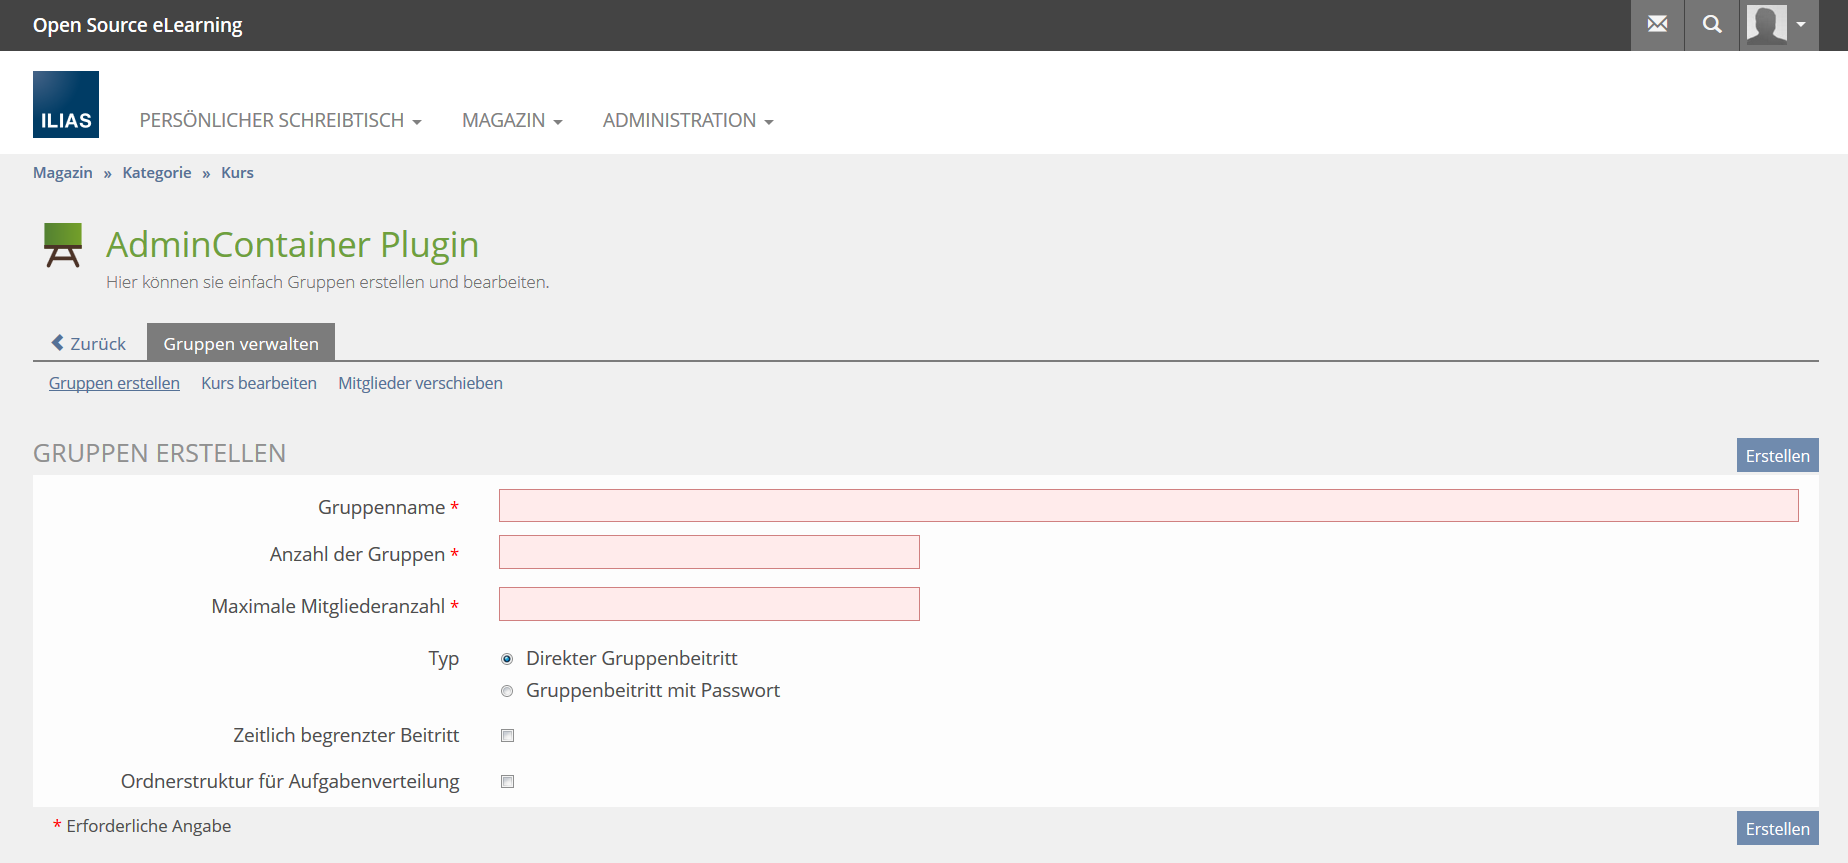
\includegraphics[width=1\textwidth]{img/gruppenErstellen.png}
	\caption{Ansicht Gruppen erstellen}
\end{figure}

In diesem Reiter/Tab lassen sich beliebig viele Gruppen erstellen. 
\newpage
\subsection*{Vorgehen - Pflichtfelder}

\begin{itemize}
	\item Eingeben eines Namenspräfix im Textfeld "Gruppennamen"  
	\item Eingeben einer Zahl größer Null im Textfeld "Anzahl der Gruppen"
	\item Eingeben einer Zahl im Textfeld "Maximale Mitgliederanzahl" für die maximale Anzahl der Gruppenmitglieder 
\end{itemize}




\subsection*{Vorgehen - optional}

\subsubsection*{Beitritts - Typ}
\begin{itemize}
	\item[1] Radiobutton auf  'Gruppenbeitritt mit Passwort'   setzen um die Gruppen mit einem Passwort zu schützen. 
	\item[2] Ein weiteres Textfeld taucht auf, bei dem das gewünschte Passwort einzugeben ist. (Passwort ist für alle in dieser Session erzeugten Gruppen dasselbe)
\end{itemize}

\subsubsection*{Zeitlich begrenzter Beitritt}
\begin{itemize}
	\item[1] Checkbox setzen 
	\item[2] Zwei Datumseingabefelder tauchen für den Anmelde-Zeitraum auf, sowohl für Beitrittsanfang und Beitrittsende einen Zeitpunkt auswählen. Format: Tag / Monat / Jahr / Stunde / Minuten 
	(Achtung, Ende kann nicht vor Start liegen)
	
\end{itemize}

\subsubsection*{Ordnerstruktur für Aufgabenverteilung}
\begin{itemize}
	\item[1] Checkbox setzen 
	\item[2] Ein Textfeld taucht auf bei dem man einen oder mehrere Ordnernamen (durch ";" getrennt) eingeben kann. Dadurch werden im Kurs als auch in allen zu erstellenden Gruppen diese Ordner mit den bzw. dem Namen erzeugt.
	
\end{itemize}
\clearpage

\section{Kurs bearbeiten}
\begin{figure}
	\centering
	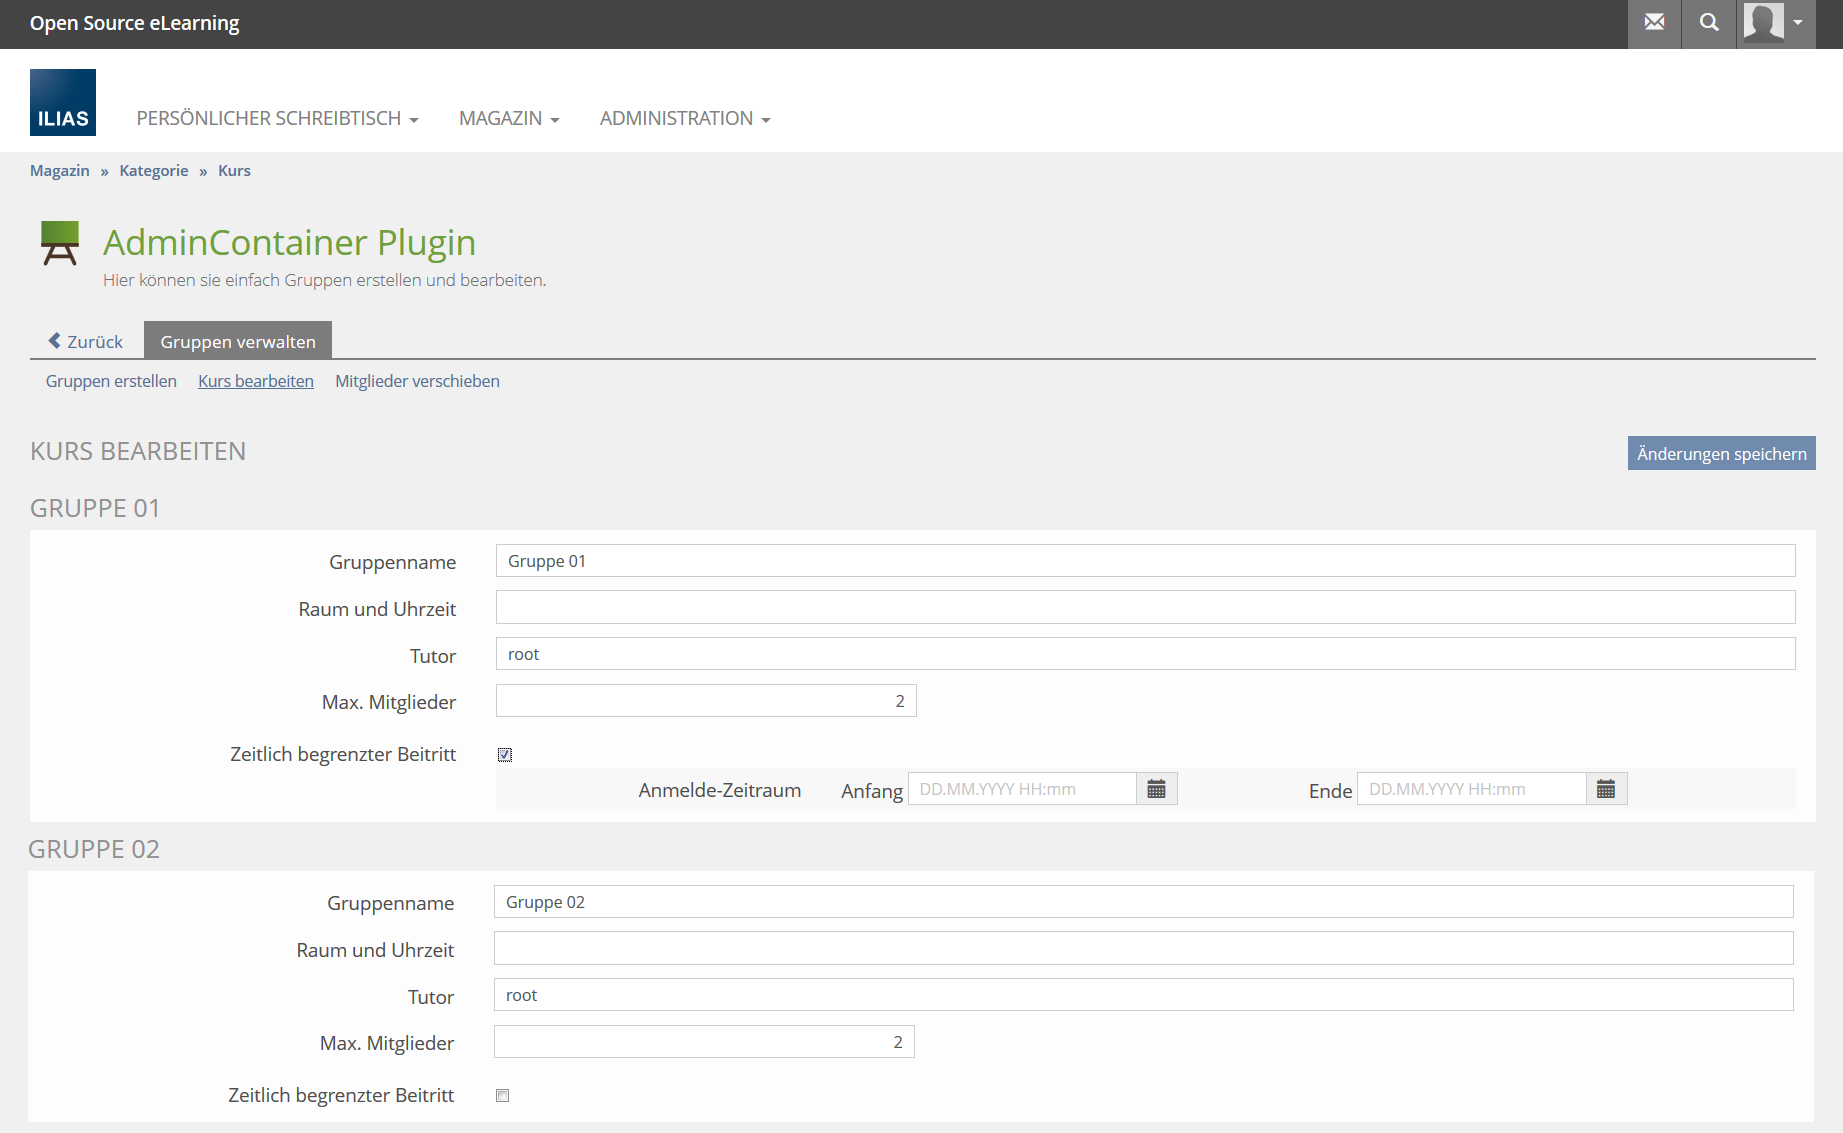
\includegraphics[width=1\textwidth]{img/kursBearbeiten.png}
	\caption{Ansicht Kurs bearbeiten}
\end{figure}

In diesem Reiter/Tab erhält man eine Übersicht aller im Kurs vorhandenen Gruppen mit folgenden Feldern. (n aus den natürlichen Zahlen)
\subsection*{Gruppen}
Die Felder können einzelnen und unabhängig voneinander bearbeitet werden. Felder zeigen den aktuellen Wert/Zustand der Gruppe an. 
Mit einem klick auf den "Änderung speichern" Knopf werden die Änderungen übernommen. 

\subsubsection{Gruppenname}
\begin{itemize}
	\item Auf das Feld klicken um den Namen verändern, dies beinhaltet den Suffix, dessen Veränderung unter Umständen die Nummerierung durcheinander bringt. (Feld darf nicht leer sein)
\end{itemize}

\subsubsection{Raum und Uhrzeit - als Beschreibung}
\begin{itemize}
	\item In das Textfeld lässt sich eine beliebige Zeichenkette eintragen (z.B. Raum und Uhrzeit), die dann als Beschreibung der Gruppe auftaucht. 
\end{itemize}

\subsubsection{Tutor}
\begin{itemize}
	\item Um der aus der Gruppe einem Mitglieder die Tutor bzw. Gruppenadministrationsrechte zuzuweisen bzw. zu entziehen. 
	\item[hinzufügen] Ilias Benutzernamen eingeben. Nach dem dritten Buchstaben funktioniert springt die Auto-Complete Funktion an und hilft beim vervollständigen. 
	\item[löschen] Sollte ein zuvor gefülltes Feld leer hinterlassen werden, werden dem Benutzer hinter dem entfernten Text die Adminrechte entzogen.
\end{itemize}

\subsubsection{Max Mitglieder}
Um den angezeigten Wert für die Gruppe zu verändern
\begin{itemize}
	\item Eingeben einer Zahl im Textfeld "Maximale Mitgliederanzahl" für die maximale Anzahl der Gruppenmitglieder 
\end{itemize}


\subsubsection{Zeitlich begrenzter Beititt}
Wenn Checkbox nicht gesetzt, gibt es keinen zeitlich begrenzten Betritt bei dieser Gruppe. Um einen zu erzeugen
\begin{itemize}
\item[1] Checkbox setzen 
\item[2] Zwei Datumseingabefelder tauchen für den Anmelde-Zeitraum auf, sowohl für Beitrittsanfang und Beitrittsende einen Zeitpunkt auswählen. Format: Tag/Monat/Jahr/Stunde/Minuten 
(Achtung, Ende kann nicht vor Start liegen)
\end{itemize}

Ansonsten Checkbox deaktivieren und begrenzter Beitritt verschwindet. 
Falls schon ausgewählt und man nur das Datum verändern will, Schritt 1 überspringen. 


\clearpage

\section{Mitglieder verschieben}
\begin{figure}
	\centering
	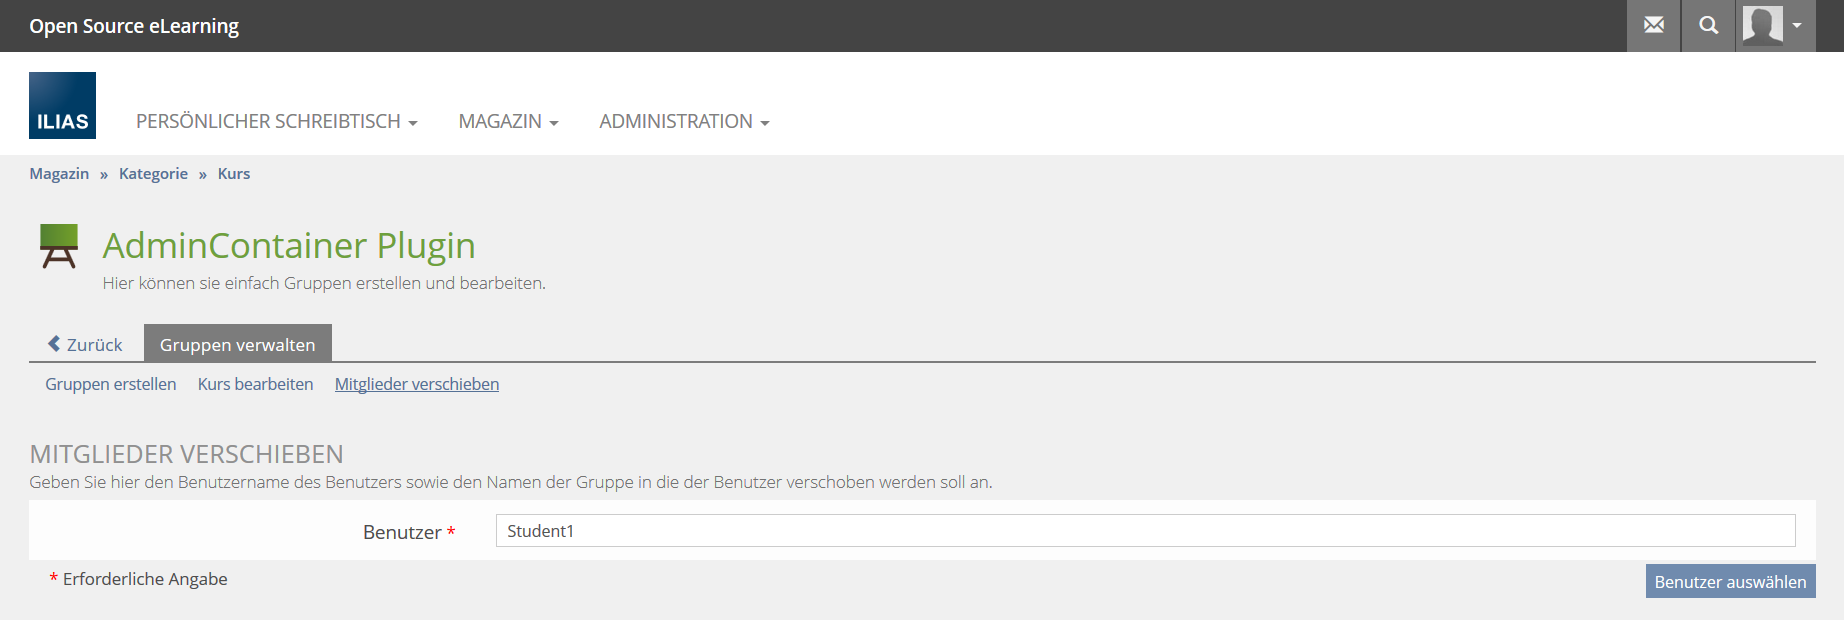
\includegraphics[width=1\textwidth]{img/mitgliederVerschieben1.png}
	\caption{Ansicht Mitglieder verschieben - Benutzer auswählen}
\end{figure}
\begin{figure}
	\centering
	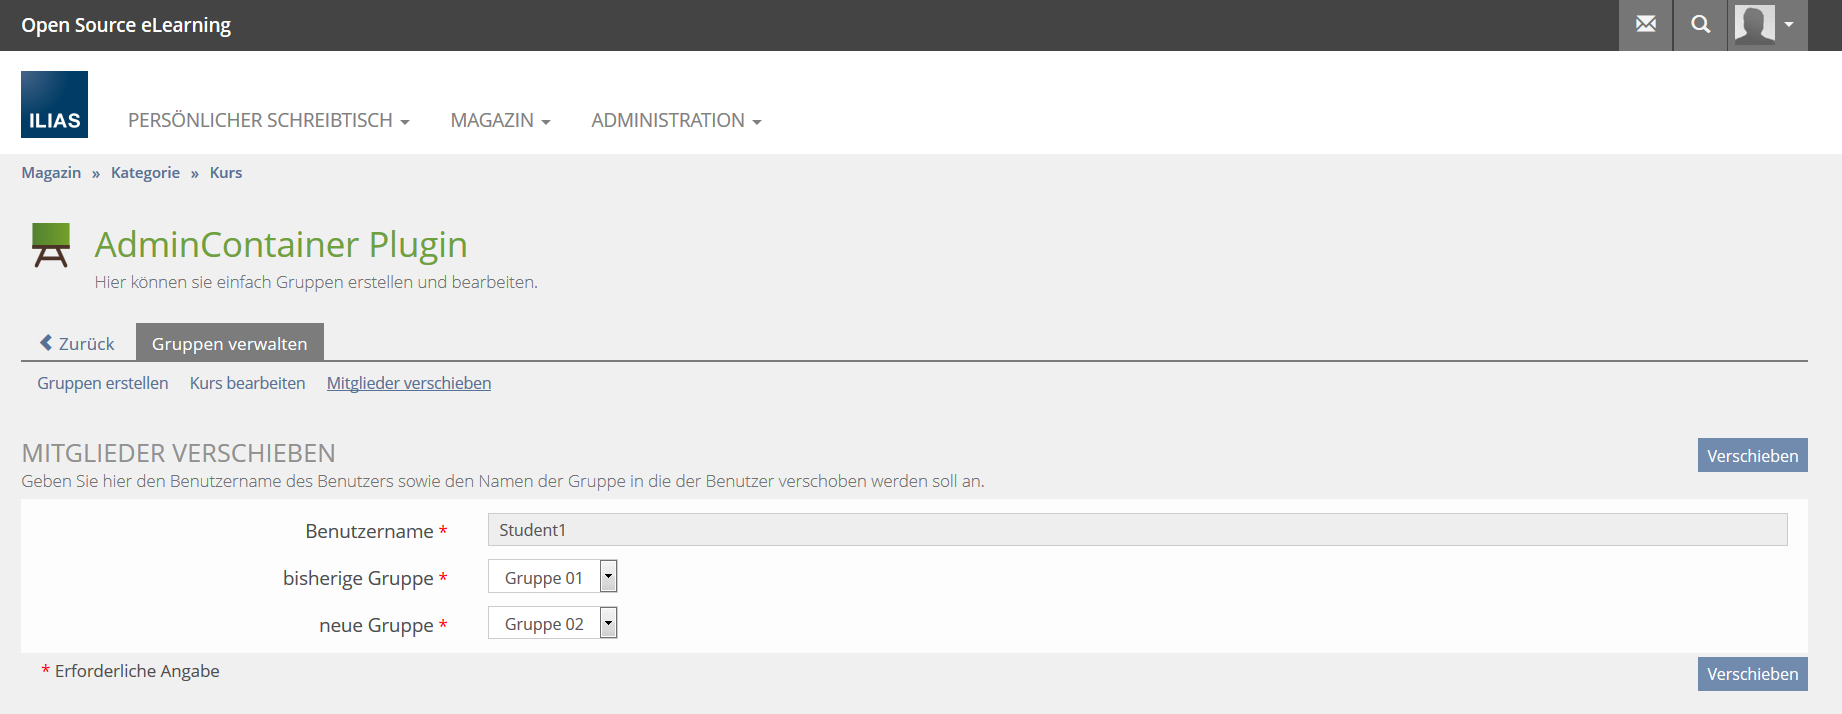
\includegraphics[width=1\textwidth]{img/mitgliederVerschieben2.png}
	\caption{Ansicht Mitglieder verschieben - Gruppen auswählen}
\end{figure}

Das Mitgliederverschieben erfolgt zweistufig. 
\subsection*{Mitglieder verschieben}
\subsubsection*{Benutzer auswählen}
\begin{itemize}
	\item Benutzernamen eingeben, ab dem dritten Buchstaben hilft die Auto-Complete Funktion beim vervollständigen. (Pflichtfeld, darf nicht leer sein)
	\item Auf "Benutzer auswählen" klicken
\end{itemize}
\subsubsection*{Benutzer wurde ausgewählt}
\begin{itemize}
	\item Auf der neuen Seite wird in dem Drop-down Menü unter "bisherige Gruppe" angezeigt in welchen Gruppen sich der Benutzer befindet, darunter unter "neue Gruppe" 
	\item Auswählen aus welcher Gruppe (Achtung im Drop-down von bisherige Gruppe Menü können mehrere Gruppen angezeigt werden, da sich Benutzer möglicherweise in mehreren Gruppen befindet)
	\item Auswählen in welche "neue Gruppe" man den Benutzer verschieben will
	\item Mit dem Klicken auf "Verschieben" die Eingabe bestätigen und den Benutzer verschieben
\end{itemize}


\clearpage